%
% the meat of the thing
%
\section{Overview}

\subsection{Background}

This project is experimenting with using a (relatively) simple set
of \ac{PERL} scripts to manage the project.  The scripts are relatively
simple, and are intended to capture the minimum of programmatic information
so as to allow the developers to develop, rather than fill their time with
bureaucratic activities.

The scripting was developed to support the \ac{APP} and makes
heavy use of the \texttt{dot} tool which is part of the \texttt{graphviz}
package developed years ago at Bell Labs.  (My speculation is that they
got started on it as part of the tool-set needed to deconstruct the original
Bell System\ldots.  My brother had a summer job working for them in that
era and did nothing but write tools to make new organization charts.)
In any case, the products of the scripts contained bubbles of activity and
were perjoratively\footnote{Shep Doeleman, 2012} termed bubble diagrams and
it's as good a description as any.  The bubbles served their purpose admirably
in convincing ALMA/NA management that we had a clue about conducting the
project.  So we shall go with a working title of ``Tasking Bubble Machine''.

In this scheme, the work of the project is partitioned into a set of large,
related areas of work called ``domains''.  Each domain is itself composed of
several threads of activity.  For want of a better term ``things'' has been
used.   Finally, at the lower level, each thing is partitioned into a set of
tasks that collectively accomplish the work.  Further decomposition into
subtasks is not considered, as different developers do that differently.

Obviously, the complexity of project management is to sort out what tasks
depend on others, match that to what is comes due at various externally
specified delivery dates, and assign effort of the development team.
The ``catch'' is that some things depend on others and sorting through
the dependencies to find the critical path---viz, the set of tasks which
ultimately determine the success or failure of the project (with respect
only to on-time completion).

The \texttt{dot} tool gets into the picture as it is very good at drawing
graphs, and (as is often said) a picture is worth a thousand words.
There are of course rather sophisticated management tools that are designed
to do these sorts of things.  The problem is that they are not simple to use
and the target user is a manager who spends alot of time pointing and clicking.

By contrast, in this scheme, the developers should be able to translate
their requirements into tasks, work out the dependencies, estimate effort,
and then let the machine tell them if the end date is going to work or not.

\textit{At this stage of development, identification of the critical path
is not captured in the scripting.  But the diagrams do indicate where the
problems are, so it should be possible to know what to think about fixing.}

\subsection{Implementation Details}

The scripts were implemented in \ac{PERL} (version 5).  Although \ac{PERL}
scripts can be written to be quite opaque, these are not.  There are even
some comments.  They read one concatenated set of input files which consist
entirely of either key = value lines, continuations (for multiple-line values)
and comments.  Some of the key = value declarations also create (automatic)
abbreviations to save repetitive typing.  Abbreviations may also be explicitly
made to, \eg capture important dates in one place.

\FIXME[continue to transcribe the material in MHO\_task\_inputs.txt]

\subsection{New HOPS Domains}

As indicated previously, the ``front matter'' is contained in the
first file (0000).  After that, there is a file that provides
information on the domains (0001).
The project to create the new \ac{MHO} has the following domains.  The
list may be generated with the command
\texttt{sw\_tasks.pl -g help -i MHO\_task.txt}, where
\texttt{MHO\_task.txt} is the concatenated input file (found in the build
directory).

% generated in the Makefile
\input{domainlist}

Each of these domains has its own section that follows this one.
The next set of files (at the moment, just 0010) contains the partition
of the domains into things.  The things are described in subsections of
the approprate domain.

The rest of the files describe the tasks in each thing.  This is shown
graphically in Fig.~\ref{fig:umlclass}.
%%%%%%%%%%%%%%%%%%%%%%%%%%%%%%%%%%%%%%%%%%%%%%%%%%%%%%%%%%%%%%%%%%%%%%%%%%%%
\begin{figure}[h!]%htbp
\captionsetup{width=0.6\linewidth}
\center{%
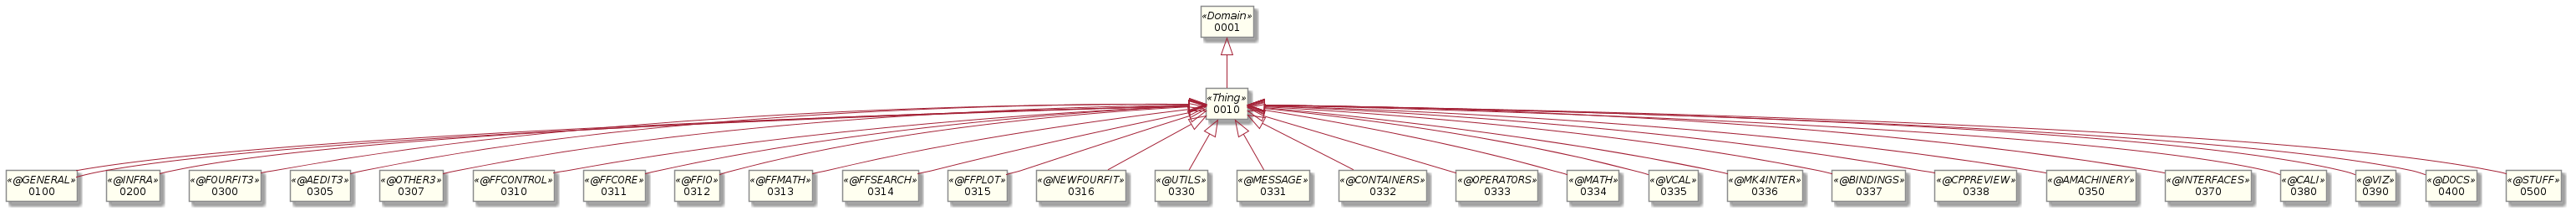
\includegraphics[width=0.7\textwidth]{plantuml-code}
\caption[Input Files]{Relationship of domains and things to input files.
Things are referenced by nickname.}}
\label{fig:umlclass}
\end{figure}
%%%%%%%%%%%%%%%%%%%%%%%%%%%%%%%%%%%%%%%%%%%%%%%%%%%%%%%%%%%%%%%%%%%%%%%%%%%%

% overview-helper.sh filename(.tex)
\subsection{Pool of Developers and Other Relevant People}
\input{devels}

\subsection{Task Definitions}
\input{taskdefs}

\subsection{Fixed Dates}
\input{dates}

%
% eof
%
